\documentclass{beamer}
\usepackage{lmodern}
\usepackage{anyfontsize}
\usepackage[T1]{fontenc}
\usepackage[italian]{babel}

\usetheme[progressbar=head]{moloch}

\setbeamertemplate{title page}{
\begin{minipage}[c][0.9\paperheight]{\textwidth} % Altezza ridotta al 90%
	\centering

	\ifx\inserttitlegraphic\@empty\else\usebeamertemplate*{title graphic}\fi
	\vfill%

	\ifx\inserttitle\@empty\else {\usebeamertemplate*{title}}\fi
	\ifx\insertsubtitle\@empty\else {\usebeamertemplate*{subtitle}}\fi

	\usebeamertemplate*{title separator}

	{
	\centering
	\ifx\beamer@shortauthor\@empty\else\usebeamertemplate*{author}\fi
	\ifx\insertdate\@empty\else\usebeamertemplate*{date}\fi
	\ifx\insertinstitute\@empty\else\usebeamertemplate*{institute}\fi
	}

	\vfill
	\vspace*{1mm}
\end{minipage}
}

\setbeamertemplate{title}{
%  \raggedright%  % <-- Comment here
  \linespread{1.0}%
  \inserttitle%
  \par%
  \vspace*{0.5em}
}

\setbeamertemplate{author}{
  \insertauthor%
  \par%
	\vspace*{0.5em}
}
%
% \setbeamerfont{footnote}{size=\small}
% \setbeamercolor{footnote}{fg=blue, bg=lightgray}
% \setbeamertemplate{footnote page}{%
%     \begin{centering}
%         \vspace{1em} \footnotesize % Puoi cambiare la dimensione del font
%         \insertfootnotetext
%     \end{centering}
% }
%
% \setbeamerfont{footnote}{size=\small}


\graphicspath{{./images}}

\usepackage[style=numeric, sorting=none]{biblatex} % Per la gestione di BibTeX
\addbibresource{slides.bib}
\usepackage{csquotes}

\AtBeginSection[]
{
  \begin{frame}
    \frametitle{Sommario}
    \tableofcontents[currentsection]
  \end{frame}
}

\AtBeginSubsection[]{
  \begin{frame}
	\frametitle{Sommario}
	\tableofcontents[currentsection,currentsubsection]
	\end{frame}
}

\usepackage{mathtools}
\usepackage{amsmath}
\newcommand{\bigo}[1]{\ensuremath{O\left({#1}\right)}}
\usepackage{booktabs}
\DeclarePairedDelimiter\bra{\langle}{\rvert}
\DeclarePairedDelimiter\ket{\lvert}{\rangle}
\DeclarePairedDelimiterX\braket[2]{\langle}{\rangle}{#1\,\delimsize\vert\,\mathopen{}#2}
\usepackage{amsmath, amssymb}

\usepackage{doi}
\usepackage{subfig}

%%%%%%%%%%%%%%%%%%%%%%%%%%%%%%%%%%%%%%%%%%%%%%%%%%%%%%%%%%%%%5


\title{Quantum Hadamard\\Edge Detection}
\author{Manuel Di Agostino}
\institute{Università di Parma}
\date{12 febbraio 2025}


\begin{document}
	\begin{frame}
		\titlepage
	\end{frame}
	\begin{frame}{Sommario}
		\tableofcontents
	\end{frame}
	
	\section{Background}


	\subsection{Edge detection}

	\begin{frame}{Edge detection}
		\begin{itemize}
			\item \textbf{Goal}: identificare oggetti in un'immagine, tramite
			\emph{contorni}
			\item Ma anche:
				\begin{itemize}
					\item estrazione di texture, pattern
					\item motion recognition
					\item image restoration
				\end{itemize}
		\end{itemize}
	\end{frame}

	\begin{frame}{Soluzioni classiche}
		\begin{figure}
			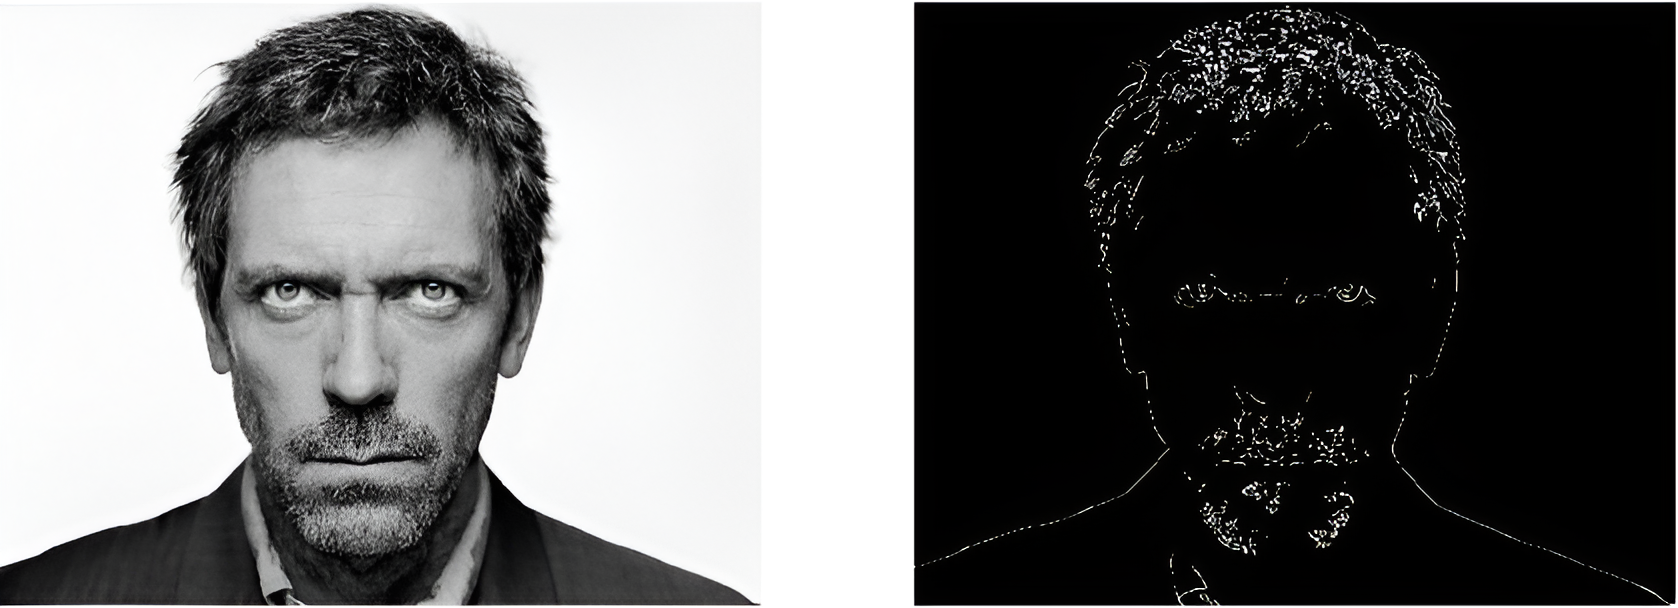
\includegraphics[width=0.9\textwidth]{edge-detection-example.png}
		\end{figure}

		\begin{itemize}
			\item Lavorano sull'immagine in scala di grigi
			\item Approssimano il gradiente dell'intensità
			\item Utilizzano operatori convolutivi (\emph{kernel})
		\end{itemize}
	\end{frame}

	\begin{frame}{Filtri di Sobel}
		\begin{itemize}
			\item Fu introdotto negli anni '60 \cite{SobelFeldman1968IsotropicGradient}
			\item Applica due kernel di convoluzione
				\[
				\mathbf{G_x} =
				\underbrace{
				\begin{bmatrix}
					+1 & 0 & -1 \\
					+2 & 0 & -2 \\
					+1 & 0 & -1
				\end{bmatrix}
				}_{\text{direzione orizzontale}}
				,\quad
				\mathbf{G_y} =
				\underbrace{
				\begin{bmatrix}
					+1 & +2 & +1 \\
					0 & 0 & 0 \\
					-1 & -2 & -1
				\end{bmatrix}
				}_{\text{direzione verticale}
				}
				\]
			\item<2-> Il nuovo valore di intensità del pixel $p_{j,k}$ è
			\[
				\tilde{p}_{j,k} = \sqrt{{G_x(p_{j,k})}^2 + {G_y(p_{j,k})}^2}
			\]
		\end{itemize}
	\end{frame}

	\begin{frame}{Filtri di Sobel}
		\begin{figure}
			\begin{center}
				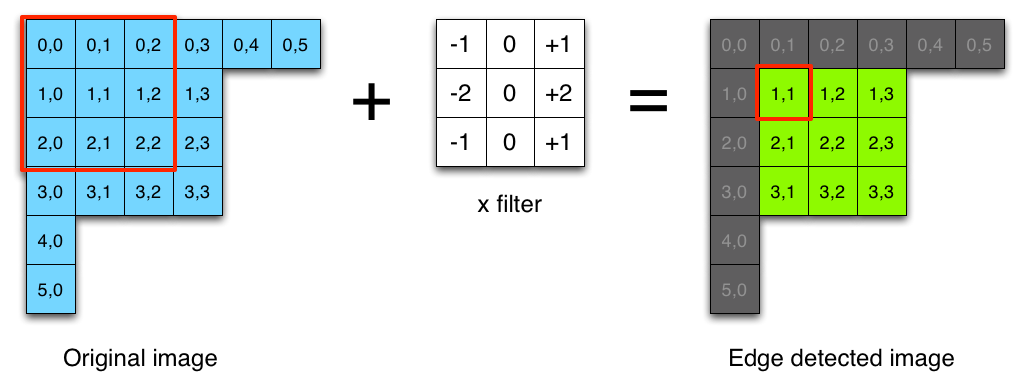
\includegraphics[width=0.9\textwidth]{sobel-appl.png}
			\end{center}
			\caption{Applicazione orizzontale del kernel di Sobel.}\label{fig:sobel-appl}
		\end{figure}
		
		\begin{itemize}
			\item Complessità \emph{lineare} rispetto al numero di pixel!
		\end{itemize}
	\end{frame}


	\subsection{Quantum computing}

	\begin{frame}{Sistemi quantistici}
		\begin{itemize}
			\item Unità  di informazione: \textbf{qubit}
			\item Notazione \emph{di Dirac}
			\[
			\ket{\psi} = \alpha\ket{0} + \beta\ket{1} = \begin{bmatrix}
				\alpha\\\beta
			\end{bmatrix},\quad \alpha,\beta \in \mathbb{C}
			\]
			\item Verificano
			\[
			|\alpha|^2 + |\beta|^2 = 1
			\]
			\pause
			\item Sistemi di più qubit descritti utilizzando il \emph{prodotto tensore}
			\[
				\ket{\psi_1} = \begin{bmatrix} a_1 \\ a_2 \end{bmatrix}, \quad \ket{\psi_2} = \begin{bmatrix} b_1 \\ b_2 \end{bmatrix},
			\]
			\[
				\ket{\psi_1} \otimes \ket{\psi_2}
				= \begin{bmatrix}
					a_1 \begin{bmatrix} b_1 \\ b_2 \end{bmatrix} \\
						a_2 \begin{bmatrix} b_1 \\ b_2 \end{bmatrix}
				\end{bmatrix} =
				\begin{bmatrix}
					a_1 b_1 \\ a_1 b_2 \\ a_2 b_1 \\ a_2 b_2
				\end{bmatrix}.
			\]
		\end{itemize}
	\end{frame}


	\subsection{Circuiti quantistici}

	\begin{frame}{Quantum gate}
		\begin{itemize}
			\item L'azione di un \textbf{quantum gate} è modellata matematicamente
			tramite l'applicazione di una matrice \emph{complessa unitaria} ad uno
			stato quantistico
			\[
			\ket{\psi'} = U\ket{\psi}
			\]
			\pause
			\item Porte rilevanti:
			\begin{itemize}
				\item Gate \emph{di Pauli}
				\[
				\sigma_x = 
				\begin{bmatrix}
					0 & 1 \\
					1 & 0
				\end{bmatrix}
				\quad
				\sigma_y = 
				\begin{bmatrix}
					0 & -i \\
					i & 0
				\end{bmatrix}
				\quad
				\sigma_z = 
				\begin{bmatrix}
					1 & 0 \\
					0 & -1
				\end{bmatrix}
				\]
				\item Gate \emph{di Hadamard}
				\[
				H = \frac{1}{\sqrt{2}}
				\begin{bmatrix}
					1 & 1 \\
					1 & -1
				\end{bmatrix}
				\]
			\end{itemize}
		\end{itemize}
	\end{frame}

	\subsection{Quantum Image Processing}

	\begin{frame}{Quantum Image Processing}
		Due obiettivi principali:
		\begin{itemize}
			\item<1-> Codifica dell'immagine nei circuiti
			\begin{itemize}
				\item Flexible Representation of Quantum Images (FRQI) \cite{Le2011}
				\item Novel Enhanced Quantum Representation (NEQR) \cite{Zhang2013}
				\item \textbf{Quantum Probability Image Encoding (QPIE)} \cite{Yao2018}
			\end{itemize}
			\item<2-> Algoritmi di processamento
			\begin{itemize}
				\item QSobel \cite{Zhang2014}
				\item \textbf{Quantum Hadamard Edge Detection (QHED)} \cite{Yao2018}
			\end{itemize}
		\end{itemize}
	\end{frame}

	\begin{frame}{Quantum Probability Image Encoding}
		\begin{itemize}
			\item Valori di intensità dei pixel codificati nelle ampiezze di
			probabilità dello stato quantistico
			\item Immagine di $N$ pixel. Qubit necessari:
			\[
				n = \lceil{log_2{N}}\rceil
			\]
		\end{itemize}
	\end{frame}

	\begin{frame}{Quantum Probability Image Encoding}
		\begin{figure}
			\centering
			\subfloat[]{
			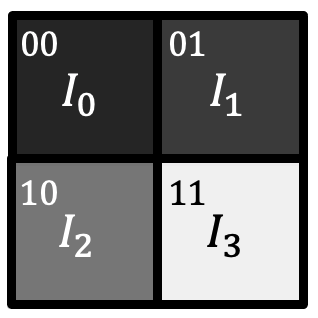
\includegraphics[width=0.25\textwidth]{classical_repr.png}\label{fig:classical_repr}
			}
			\subfloat[]{
			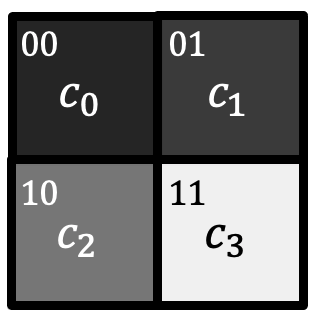
\includegraphics[width=0.25\textwidth]{QPIE_repr.png}\label{fig:QPIE_repr}
			}
			\caption{(\ref{fig:classical_repr}) rappresentazione classica, (\ref{fig:QPIE_repr}) rappresentazione quantistica.}
		\end{figure}

		\begin{itemize}
			\item Pixel numerati utilizando stringhe binarie
			\item Intensità normalizzate secondo
			\[
				c_i = \frac{I_i}{\sqrt{\sum_{k}^{}{I_{k}^2}}}
			\]
		\end{itemize}
	\end{frame}

	\begin{frame}{Quantum Probability Image Encoding}
		\begin{itemize}
			\item Nell'esempio
			(\ref{fig:QPIE_repr})
			si ottiene
			\[
			\ket{\text{Img}} 
				= c_0 \ket{00} + c_1 \ket{01} + c_2 \ket{10} + c_3 \ket{11}
				= \begin{bmatrix}
					c_0\\c_1\\c_2\\c_3
				\end{bmatrix}
			\]
			\pause
			\item Generalizzando per $n$ qubit
			\[
				\ket{\text{Img}} 
					= \sum_{i=1}^{2^n} c_i \ket{i}
					= \begin{bmatrix}
						c_0\\c_1\\ \vdots\\c_{N-2}\\c_{N-1}
				\end{bmatrix}
			\]
		\end{itemize}

	\end{frame}

	\begin{frame}[allowframebreaks]{Quantum Hadamard Edge Detection}
		\begin{itemize}
			\item Fa uso della QPIE
			\item \textbf{Idea di base}: utilizzare il \emph{gate di Hadamard} sul qubit $q_0$
			\[
			I_{2^{n-1}} \otimes H_0 = \frac{1}{\sqrt 2}\begin{bmatrix}
				1 & 1 & 0 & 0 & \ldots & 0 & 0\\
				1 & -1 & 0 & 0 & \ldots & 0 & 0\\
				0 & 0 & 1 & 1 & \ldots & 0 & 0\\
				0 & 0 & 1 & -1 & \ldots & 0 & 0\\
				\vdots & \vdots & \vdots & \vdots & \ddots & \vdots & \vdots\\
				0 & 0 & 0 & 0 & \ldots & 1 & 1\\
				0 & 0 & 0 & 0 & \ldots & 1 & -1\\
			\end{bmatrix}
			\]
			\item Applicando questa trasformazione a $\ket{\text{Img}}$ si ottiene lo
			stato
			\[
			(I_{2^{n-1}} \otimes H_0) \cdot \begin{bmatrix}
				c_0\\ c_1\\ c_2\\ c_3\\ \vdots\\ c_{N-2}\\ c_{N-1}
			\end{bmatrix} = \frac{1}{\sqrt 2} \begin{bmatrix}
				c_0+c_1\\ c_0-c_1\\ c_2+c_3\\ c_2-c_3\\ \vdots\\ c_{N-2}+c_{N-1}\\ c_{N-2}-c_{N-1}
			\end{bmatrix}
			\]
			che esplicita il gradiente di coppie (\emph{pari}) di
			pixel adiacenti
			\item Questo è riconducibile a
			\[
			\frac{1}{\sqrt 2} (\ket{\text{sum}} \otimes \ket{0}
			+ \ket{\text{dif}} \otimes \ket{1})
			\]
			\item \textbf{Punto chiave}: misurare il circuito a condizione che $q_0$
			sia nello stato $\ket{1}$
		\end{itemize}
	\end{frame}


	\section{Implementazione}

	\section{Risultati}

	\section{Conclusione}

	\begin{frame}[allowframebreaks]{Bibliografia}
		\printbibliography
	\end{frame}

\end{document}
